\chapter{廣度優先搜索}
當題目看不出任何規律,既不能用分治,貪心,也不能用動規時,這時候萬能方法——搜索,
就派上用場了。搜索分為廣搜和深搜,廣搜裏面又有普通廣搜,雙向廣搜,A*搜索等。
深搜裏面又有普通深搜,回溯法等。

廣搜和深搜非常類似(除了在擴展節點這部分不一樣),二者有相同的框架,如何表示狀態?
如何擴展狀態?如何判重?尤其是判重,解決了這個問題,基本上整個問題就解決了。
\newline


\section{Word Ladder} %%%%%%%%%%%%%%%%%%%%%%%%%%%%%%
\label{sec:word-ladder}


\subsubsection{描述}
Given two words (start and end), and a dictionary, find the length of shortest transformation sequence from start to end, such that:
\begindot
\item Only one letter can be changed at a time
\item Each intermediate word must exist in the dictionary
\myenddot

For example, Given:

\begin{Code}
start = "hit"
end = "cog"
dict = ["hot","dot","dog","lot","log","cog"]
\end{Code}
As one shortest transformation is \code{"hit" -> "hot" -> "dot" -> "dog" -> "cog"}, return its length $5$.

Note:
\begindot
\item Return 0 if there is no such transformation sequence.
\item All words have the same length.
\item All words contain only lowercase alphabetic characters.
\myenddot


\subsubsection{分析}
求最短路徑,用廣搜。


\subsubsection{單隊列}
\begin{Code}
//LeetCode, Word Ladder
// 時間複雜度O(n),空間複雜度O(n)
struct state_t {
    string word;
    int level;

    state_t() { word = ""; level = 0; }
    state_t(const string& word, int level) {
        this->word = word;
        this->level = level;
    }

    bool operator==(const state_t &other) const {
        return this->word == other.word;
    }
};

namespace std {
    template<> struct hash<state_t> {
    public:
        size_t operator()(const state_t& s) const {
            return str_hash(s.word);
        }
    private:
        std::hash<std::string> str_hash;
    };
}


class Solution {
public:
    int ladderLength(const string& start, const string &end,
            const unordered_set<string> &dict) {
        queue<state_t> q;
        unordered_set<state_t> visited;  // 判重

        auto state_is_valid = [&](const state_t& s) {
            return dict.find(s.word) != dict.end();
        };
        auto state_is_target = [&](const state_t &s) {return s.word == end; };
        auto state_extend = [&](const state_t &s) {
            unordered_set<state_t> result;

            for (size_t i = 0; i < s.word.size(); ++i) {
                state_t new_state(s.word, s.level + 1);
                for (char c = 'a'; c <= 'z'; c++) {
                    // 防止同字母替換
                    if (c == new_state.word[i]) continue;

                    swap(c, new_state.word[i]);

                    if (state_is_valid(new_state) &&
                        visited.find(new_state) == visited.end()) {
                        result.insert(new_state);
                    }
                    swap(c, new_state.word[i]); // 恢復該單詞
                }
            }

            return result;
        };

        state_t start_state(start, 0);
        q.push(start_state);
        visited.insert(start_state);
        while (!q.empty()) {
            // 千萬不能用 const auto&,pop() 會刪除元素,
            // 引用就變成了懸空引用
            const auto state = q.front();
            q.pop();

            if (state_is_target(state)) {
                return state.level + 1;
            }

            const auto& new_states = state_extend(state);
            for (const auto& new_state : new_states) {
                q.push(new_state);
                visited.insert(new_state);
            }
        }
        return 0;
    }
};
\end{Code}


\subsubsection{雙隊列}
\begin{Code}
//LeetCode, Word Ladder
// 時間複雜度O(n),空間複雜度O(n)
class Solution {
public:
    int ladderLength(const string& start, const string &end,
            const unordered_set<string> &dict) {
        queue<string> current, next;    // 當前層,下一層
        unordered_set<string> visited;  // 判重

        int level = -1;  // 層次

        auto state_is_valid = [&](const string& s) {
            return dict.find(s) != dict.end();
        };
        auto state_is_target = [&](const string &s) {return s == end;};
        auto state_extend = [&](const string &s) {
            unordered_set<string> result;

            for (size_t i = 0; i < s.size(); ++i) {
                string new_word(s);
                for (char c = 'a'; c <= 'z'; c++) {
                    // 防止同字母替換
                    if (c == new_word[i]) continue;

                    swap(c, new_word[i]);

                    if (state_is_valid(new_word) &&
                        visited.find(new_word) == visited.end()) {
                        result.insert(new_word);
                    }
                    swap(c, new_word[i]); // 恢復該單詞
                }
            }

            return result;
        };

        current.push(start);
        visited.insert(start);
        while (!current.empty()) {
            ++level;
            while (!current.empty()) {
                // 千萬不能用 const auto&,pop() 會刪除元素,
                // 引用就變成了懸空引用
                const auto state = current.front();
                current.pop();

                if (state_is_target(state)) {
                    return level + 1;
                }

                const auto& new_states = state_extend(state);
                for (const auto& new_state : new_states) {
                    next.push(new_state);
                    visited.insert(new_state);
                }
            }
            swap(next, current);
        }
        return 0;
    }
};
\end{Code}


\subsubsection{相關題目}

\begindot
\item Word Ladder II,見 \S \ref{sec:word-ladder-ii}
\myenddot


\section{Word Ladder II} %%%%%%%%%%%%%%%%%%%%%%%%%%%%%%
\label{sec:word-ladder-ii}


\subsubsection{描述}
Given two words (start and end), and a dictionary, find all shortest transformation sequence(s) from start to end, such that:
\begindot
\item Only one letter can be changed at a time
\item Each intermediate word must exist in the dictionary
\myenddot

For example, Given:
\begin{Code}
start = "hit"
end = "cog"
dict = ["hot","dot","dog","lot","log"]
\end{Code}
Return
\begin{Code}
[
    ["hit","hot","dot","dog","cog"],
    ["hit","hot","lot","log","cog"]
]
\end{Code}

Note:
\begindot
\item All words have the same length.
\item All words contain only lowercase alphabetic characters.
\myenddot


\subsubsection{分析}
跟 Word Ladder比,這題是求路徑本身,不是路徑長度,也是BFS,略微麻煩點。

求一條路徑和求所有路徑有很大的不同,求一條路徑,每個狀態節點只需要記錄一個前驅即可;求所有路徑時,有的狀態節點可能有多個父節點,即要記錄多個前驅。

如果當前路徑長度已經超過當前最短路徑長度,可以中止對該路徑的處理,因為我們要找的是最短路徑。


\subsubsection{單隊列}

\begin{Code}
//LeetCode, Word Ladder II
// 時間複雜度O(n),空間複雜度O(n)
struct state_t {
    string word;
    int level;

    state_t() { word = ""; level = 0; }
    state_t(const string& word, int level) {
        this->word = word;
        this->level = level;
    }

    bool operator==(const state_t &other) const {
        return this->word == other.word;
    }
};

namespace std {
    template<> struct hash<state_t> {
    public:
        size_t operator()(const state_t& s) const {
            return str_hash(s.word);
        }
    private:
        std::hash<std::string> str_hash;
    };
}


class Solution {
public:
    vector<vector<string> > findLadders(const string& start,
        const string& end, const unordered_set<string> &dict) {
        queue<state_t> q;
        unordered_set<state_t> visited; // 判重
        unordered_map<state_t, vector<state_t> > father; // DAG (樹) key: child value: father

        auto state_is_valid = [&](const state_t& s) {
            return dict.find(s.word) != dict.end();
        };
        auto state_is_target = [&](const state_t &s) {return s.word == end; };
        auto state_extend = [&](const state_t &s) {
            unordered_set<state_t> result;

            for (size_t i = 0; i < s.word.size(); ++i) {
                state_t new_state(s.word, s.level + 1);
                for (char c = 'a'; c <= 'z'; c++) {
                    // 防止同字母替換
                    if (c == new_state.word[i]) continue;

                    swap(c, new_state.word[i]);

                    if (state_is_valid(new_state)) {
                        auto visited_iter = visited.find(new_state);

                        if (visited_iter != visited.end()) {
                            if (visited_iter->level < new_state.level) {
                                // do nothing
                            } else if (visited_iter->level == new_state.level) {
                                result.insert(new_state);
                            } else { // not possible
                                throw std::logic_error("not possible to get here");
                            }
                        } else {
                            result.insert(new_state);
                        }
                    }
                    swap(c, new_state.word[i]); // 恢復該單詞
                }
            }

            return result;
        };

        vector<vector<string>> result;
        state_t start_state(start, 0);
        q.push(start_state);
        visited.insert(start_state);
        while (!q.empty()) {
            // 千萬不能用 const auto&,pop() 會刪除元素,
            // 引用就變成了懸空引用
            const auto state = q.front();
            q.pop();

            // 如果當前路徑長度已經超過當前最短路徑長度,
            // 可以中止對該路徑的處理,因為我們要找的是最短路徑
            if (!result.empty() && state.level + 1 > result[0].size()) break;

            if (state_is_target(state)) {
                vector<string> path;
                gen_path(father, start_state, state, path, result);
                continue;
            }
            // 必須挪到下面,比如同一層A和B兩個節點均指向了目標節點,
            // 那麼目標節點就會在q中出現兩次,輸出路徑就會翻倍
            // visited.insert(state);

            // 擴展節點
            const auto& new_states = state_extend(state);
            for (const auto& new_state : new_states) {
                if (visited.find(new_state) == visited.end()) {
                    q.push(new_state);
                }
                visited.insert(new_state);
                father[new_state].push_back(state);
            }
        }

        return result;
    }
private:
    void gen_path(unordered_map<state_t, vector<state_t> > &father,
        const state_t &start, const state_t &state, vector<string> &path,
        vector<vector<string> > &result) {
        path.push_back(state.word);
        if (state == start) {
            if (!result.empty()) {
                if (path.size() < result[0].size()) {
                    result.clear();
                    result.push_back(path);
                    reverse(result.back().begin(), result.back().end());
                } else if (path.size() == result[0].size()) {
                    result.push_back(path);
                    reverse(result.back().begin(), result.back().end());
                } else { // not possible
                    throw std::logic_error("not possible to get here ");
                }
            } else {
                result.push_back(path);
                reverse(result.back().begin(), result.back().end());
            }

        } else {
            for (const auto& f : father[state]) {
                gen_path(father, start, f, path, result);
            }
        }
        path.pop_back();
    }
};
\end{Code}


\subsubsection{雙隊列}

\begin{Code}
//LeetCode, Word Ladder II
// 時間複雜度O(n),空間複雜度O(n)
class Solution {
public:
    vector<vector<string> > findLadders(const string& start,
            const string& end, const unordered_set<string> &dict) {
        // 當前層,下一層,用unordered_set是為了去重,例如兩個父節點指向
        // 同一個子節點,如果用vector, 子節點就會在next裏出現兩次,其實此
        // 時 father 已經記錄了兩個父節點,next裏重複出現兩次是沒必要的
        unordered_set<string> current, next;
        unordered_set<string> visited; // 判重
        unordered_map<string, vector<string> > father; // DAG

        int level = -1;  // 層次

        auto state_is_valid = [&](const string& s) {
            return dict.find(s) != dict.end();
        };
        auto state_is_target = [&](const string &s) {return s == end;};
        auto state_extend = [&](const string &s) {
            unordered_set<string> result;

            for (size_t i = 0; i < s.size(); ++i) {
                string new_word(s);
                for (char c = 'a'; c <= 'z'; c++) {
                    // 防止同字母替換
                    if (c == new_word[i]) continue;

                    swap(c, new_word[i]);

                    if (state_is_valid(new_word) &&
                            visited.find(new_word) == visited.end()) {
                        result.insert(new_word);
                    }
                    swap(c, new_word[i]); // 恢復該單詞
                }
            }

            return result;
        };

        vector<vector<string> > result;
        current.insert(start);
        while (!current.empty()) {
            ++ level;
            // 如果當前路徑長度已經超過當前最短路徑長度,可以中止對該路徑的
            // 處理,因為我們要找的是最短路徑
            if (!result.empty() && level+1 > result[0].size()) break;

            // 1. 延遲加入visited, 這樣才能允許兩個父節點指向同一個子節點
            // 2. 一股腦current 全部加入visited, 是防止本層前一個節點擴展
            // 節點時,指向了本層後面尚未處理的節點,這條路徑必然不是最短的
            for (const auto& state : current)
                visited.insert(state);
            for (const auto& state : current) {
                if (state_is_target(state)) {
                    vector<string> path;
                    gen_path(father, path, start, state, result);
                    continue;
                }

                const auto new_states = state_extend(state);
                for (const auto& new_state : new_states) {
                    next.insert(new_state);
                    father[new_state].push_back(state);
                }
            }

            current.clear();
            swap(current, next);
        }

        return result;
    }
private:
    void gen_path(unordered_map<string, vector<string> > &father,
            vector<string> &path, const string &start, const string &word,
            vector<vector<string> > &result) {
        path.push_back(word);
        if (word == start) {
            if (!result.empty()) {
                if (path.size() < result[0].size()) {
                    result.clear();
                    result.push_back(path);
                } else if(path.size() == result[0].size()) {
                    result.push_back(path);
                } else {
                    // not possible
                    throw std::logic_error("not possible to get here");
                }
            } else {
                result.push_back(path);
            }
            reverse(result.back().begin(), result.back().end());
        } else {
            for (const auto& f : father[word]) {
                gen_path(father, path, start, f, result);
            }
        }
        path.pop_back();
    }
};
\end{Code}


\subsubsection{圖的廣搜}

本題還可以看做是圖上的廣搜。給定了字典 \fn{dict},可以基於它畫出一個無向圖,表示單詞之間可以互相轉換。本題的本質就是已知起點和終點,在圖上找出所有最短路徑。

\begin{Code}
//LeetCode, Word Ladder II
// 時間複雜度O(n),空間複雜度O(n)
class Solution {
public:
    vector<vector<string> > findLadders(const string& start,
            const string &end, const unordered_set<string> &dict) {
        const auto& g = build_graph(dict);
        vector<state_t*> pool;
        queue<state_t*> q; // 未處理的節點
        // value 是所在層次
        unordered_map<string, int> visited;

        auto state_is_target = [&](const state_t *s) {return s->word == end; };

        vector<vector<string>> result;
        q.push(create_state(nullptr, start, 0, pool));
        while (!q.empty()) {
            state_t* state = q.front();
            q.pop();

            // 如果當前路徑長度已經超過當前最短路徑長度,
            // 可以中止對該路徑的處理,因為我們要找的是最短路徑
            if (!result.empty() && state->level+1 > result[0].size()) break;

            if (state_is_target(state)) {
                const auto& path = gen_path(state);
                if (result.empty()) {
                    result.push_back(path);
                } else {
                    if (path.size() < result[0].size()) {
                        result.clear();
                        result.push_back(path);
                    } else if (path.size() == result[0].size()) {
                        result.push_back(path);
                    } else {
                        // not possible
                        throw std::logic_error("not possible to get here");
                    }
                }
                continue;
            }

            // 擴展節點
            auto iter = g.find(state->word);
            if (iter == g.end()) continue;

            for (const auto& neighbor : iter->second) {
                auto visited_iter = visited.find(neighbor);

                if (visited_iter != visited.end() && 
                    visited_iter->second < state->level + 1) {
                    continue;
                }

                visited[neighbor] = state->level;
                q.push(create_state(state, neighbor, state->level + 1, pool));
            }
        }

        // release all states
        for (auto state : pool) {
            delete state;
        }
        return result;
    }

private:
    struct state_t {
        state_t* father;
        string word;
        int level; // 所在層次,從0開始編號

        state_t(state_t* father_, const string& word_, int level_) :
            father(father_), word(word_), level(level_) {}
    };

    state_t* create_state(state_t* parent, const string& value,
            int length, vector<state_t*>& pool) {
        state_t* node = new state_t(parent, value, length);
        pool.push_back(node);

        return node;
    }
    vector<string> gen_path(const state_t* node) {
        vector<string> path;

        while(node != nullptr) {
            path.push_back(node->word);
            node = node->father;
        }

        reverse(path.begin(), path.end());
        return path;
    }

    unordered_map<string, unordered_set<string> > build_graph(
            const unordered_set<string>& dict) {
        unordered_map<string, unordered_set<string> > adjacency_list;

        for (const auto& word : dict) {
            for (size_t i = 0; i < word.size(); ++i) {
                string new_word(word);
                for (char c = 'a'; c <= 'z'; c++) {
                    // 防止同字母替換
                    if (c == new_word[i]) continue;

                    swap(c, new_word[i]);

                    if ((dict.find(new_word) != dict.end())) {
                        auto iter = adjacency_list.find(word);
                        if (iter != adjacency_list.end()) {
                            iter->second.insert(new_word);
                        } else {
                            adjacency_list.insert(pair<string,
                                unordered_set<string>>(word, unordered_set<string>()));
                            adjacency_list[word].insert(new_word);
                        }
                    }
                    swap(c, new_word[i]); // 恢復該單詞
                }
            }
        }
        return adjacency_list;
    }
};
\end{Code}


\subsubsection{相關題目}

\begindot
\item Word Ladder,見 \S \ref{sec:word-ladder}
\myenddot


\section{Surrounded Regions} %%%%%%%%%%%%%%%%%%%%%%%%%%%%%%
\label{sec:surrounded-regions}


\subsubsection{描述}
Given a 2D board containing \fn{'X'} and \fn{'O'}, capture all regions surrounded by \fn{'X'}.

A region is captured by flipping all \fn{'O'}s into \fn{'X'}s in that surrounded region .

For example,
\begin{Code}
X X X X
X O O X
X X O X
X O X X
\end{Code}

After running your function, the board should be:
\begin{Code}
X X X X
X X X X
X X X X
X O X X
\end{Code}


\subsubsection{分析}
廣搜。從上下左右四個邊界往裏走,凡是能碰到的\fn{'O'},都是跟邊界接壤的,應該保留。


\subsubsection{代碼}
\begin{Code}
// LeetCode, Surrounded Regions
// BFS,時間複雜度O(n),空間複雜度O(n)
class Solution {
public:
    void solve(vector<vector<char>> &board) {
        if (board.empty()) return;

        const int m = board.size();
        const int n = board[0].size();
        for (int i = 0; i < n; i++) {
            bfs(board, 0, i);
            bfs(board, m - 1, i);
        }
        for (int j = 1; j < m - 1; j++) {
            bfs(board, j, 0);
            bfs(board, j, n - 1);
        }
        for (int i = 0; i < m; i++)
            for (int j = 0; j < n; j++)
                if (board[i][j] == 'O')
                    board[i][j] = 'X';
                else if (board[i][j] == '+')
                    board[i][j] = 'O';
    }
private:
    void bfs(vector<vector<char>> &board, int i, int j) {
        typedef pair<int, int> state_t;
        queue<state_t> q;
        const int m = board.size();
        const int n = board[0].size();

        auto state_is_valid = [&](const state_t &s) {
            const int x = s.first;
            const int y = s.second;
            if (x < 0 || x >= m || y < 0 || y >= n || board[x][y] != 'O')
                return false;
            return true;
        };

        auto state_extend = [&](const state_t &s) {
            vector<state_t> result;
            const int x = s.first;
            const int y = s.second;
            // 上下左右
            const state_t new_states[4] = {{x-1,y}, {x+1,y},
                    {x,y-1}, {x,y+1}};
            for (int k = 0; k < 4;  ++k) {
                if (state_is_valid(new_states[k])) {
                    // 既有標記功能又有去重功能
                    board[new_states[k].first][new_states[k].second] = '+';
                    result.push_back(new_states[k]);
                }
            }

            return result;
        };

        state_t start = { i, j };
        if (state_is_valid(start)) {
            board[i][j] = '+';
            q.push(start);
        }
        while (!q.empty()) {
            auto cur = q.front();
            q.pop();
            auto new_states = state_extend(cur);
            for (auto s : new_states) q.push(s);
        }
    }
};
\end{Code}


\subsubsection{相關題目}

\begindot
\item 無
\myenddot

\section{Walls and Gates}
\label{sec:walls-and-gates}

\subsubsection{描述}
You are given a m x n 2D grid initialized with these three possible values.

\begindot
\item -1 - A wall or an obstacle.
\item 0 - A gate.
\item INF - Infinity means an empty room. We use the value 231 - 1 = 2147483647 to represent INF as you may assume that the distance to a gate is less than 2147483647.
\myenddot

Fill each empty room with the distance to its nearest gate. If it is impossible to reach a gate, it should be filled with INF.

Example:
Given the 2D grid:
\begin{Code}
INF  -1  0  INF
INF INF INF  -1
INF  -1 INF  -1
  0  -1 INF INF
\end{Code}

After running your function, the 2D grid should be:
\begin{Code}
  3  -1   0   1
  2   2   1  -1
  1  -1   2  -1
  0  -1   3   4
\end{Code}


\subsubsection{BFS}
\begin{Code}
// LeetCode
// 時間複雜度O(n*m),空間複雜度O(1)
int rows[] = {0, 0, 1,-1};
int cols[] = {1,-1, 0, 0};
#define INF 2147483647
class Solution {
public:
    bool isSafe(vector<vector<int>>& rooms,int i, int j)
    {
        if( i <0 or i>=rooms.size() or j <0 or j >= rooms[0].size() or rooms[i][j] != INF )
            return false;
        return true;
    }

    void wallsAndGates(vector<vector<int>>& rooms) {
        int r = rooms.size();
        if (r < 1) return;
        int c = rooms[0].size();
        queue<pair<int,int>> q;
        for (int i=0; i < r; i++)
            for(int j=0; j <c; j++)
                if (rooms[i][j]==0)
                    q.push({i, j}); // 由每一個閘口開始

        while(!q.empty())
        {
            auto p = q.front(); q.pop();

            for(int d=0; d<4; d++)
            {
                int x = p.first  + rows[d];
                int y = p.second + cols[d];
                if (isSafe(rooms,x,y) )
                {
                    rooms[x][y] =  rooms[p.first][p.second] + 1;
                    q.push({x,y});
                }
            }
        }
    }
};
\end{Code}

\section{Open the Lock}
\label{sec:open-the-lock}

\subsection{描述}
You have a lock in front of you with 4 circular wheels. Each wheel has 10 slots: '0', '1', '2', '3', '4', '5', '6', '7', '8', '9'. The wheels can rotate freely and wrap around: for example we can turn '9' to be '0', or '0' to be '9'. Each move consists of turning one wheel one slot.

The lock initially starts at '0000', a string representing the state of the 4 wheels.

You are given a list of deadends dead ends, meaning if the lock displays any of these codes, the wheels of the lock will stop turning and you will be unable to open it.

Given a target representing the value of the wheels that will unlock the lock, return the minimum total number of turns required to open the lock, or -1 if it is impossible.

Example 1:
\begin{Code}
Input: deadends = ["0201","0101","0102","1212","2002"], target = "0202"
Output: 6
Explanation:
A sequence of valid moves would be "0000" -> "1000" -> "1100" -> "1200" -> "1201" -> "1202" -> "0202".
Note that a sequence like "0000" -> "0001" -> "0002" -> "0102" -> "0202" would be invalid,
because the wheels of the lock become stuck after the display becomes the dead end "0102".
\end{Code}

Example 2:
\begin{Code}
Input: deadends = ["8888"], target = "0009"
Output: 1
Explanation:
We can turn the last wheel in reverse to move from "0000" -> "0009".
\end{Code}

Example 3:
\begin{Code}
Input: deadends = ["8887","8889","8878","8898","8788","8988","7888","9888"], target = "8888"
Output: -1
Explanation:
We can't reach the target without getting stuck.
\end{Code}

Example 4:
\begin{Code}
Input: deadends = ["0000"], target = "8888"
Output: -1
\end{Code}

\begindot
\item The length of deadends will be in the range [1, 500].
\item target will not be in the list deadends.
\item Every string in deadends and the string target will be a string of 4 digits from the 10,000 possibilities '0000' to '9999'.
\myenddot

\subsection{分析}
Nil

\subsection{BFS}
\begin{Code}
// LeetCode
// 時間複雜度O(N^2 * A^N + D),空間複雜度O(A^N + D)
// D is the size of deadends, A is the number of digits in our alphabet
// N is the number of digits
class Solution {
public:
    int openLock(vector<string>& deadends, string target) {
        unordered_set<string> deadendsMap(deadends.begin(), deadends.end());
        unordered_set<string> visited;

        queue<pair<string, int>> q;
        q.push({"0000", 0});

        int level = 0;
        while (!q.empty())
        {
            auto cur = q.front();
            q.pop();

            // 到了 dead end 處理下一個
            if (deadendsMap.find(cur.first) != deadendsMap.end()) continue;
            // 找到了答案
            if (cur.first == target) return cur.second;

            for (const auto& nextPW : GetNextPW(cur.first, visited))
            {
                visited.insert(nextPW);
                q.push({nextPW, cur.second + 1});
            }
        }

        return -1;
    }
private:
    const vector<int> steps{-1, 1};

    vector<string> GetNextPW(string curPW, const unordered_set<string>& visited)
    {
        vector<string> result; result.reserve(curPW.size() * 2);
        for (char& c : curPW)
        {
            char prev = c;
            for (const auto& n : steps)
            {
                c = ((10 + c - '0' + n) % 10) + '0';
                if (visited.find(curPW) == visited.end())
                    result.push_back(curPW);
                c = prev;
            }
        }

        return result;
    }
};
\end{Code}

\subsection{Counting}
\begin{Code}
// LeetCode
// 時間複雜度O(),空間複雜度O()
class Solution {
public:
    int openLock(vector<string>& deadends, string target) {
        vector<int> bucket(10000, 0);
        vector<int> rotate = { 0, 1, 2, 3, 4, 5, 4, 3, 2, 1 };
        for (auto& s : deadends) {
            bucket[stoi(s)] = 1;
        }

        if (1 == bucket[0]) return -1;

        vector<string> diffOne;

        for (int i = 0; i < 4; ++i) {
            diffOne.push_back(add(target, i, -1));
            diffOne.push_back(add(target, i, 1));
        }

        int ans = numeric_limits<int>::max();

        for (auto& s : diffOne) {
            if (0 == bucket[stoi(s)]) {
                ans = min(ans, moves(s, rotate) + 1);
            }
        }

        if (ans == numeric_limits<int>::max()) ans = -1;

        return ans;
    }

private:
    string add(const string& num, int idx, int delta)
    {
        string ans = num;
        char ch = num[idx];

        if ('0' == ch && delta == -1) {
            ans[idx] = '9';
        }
        else if ('9' == ch && delta == 1) {
            ans[idx] = '0';
        }
        else {
            ans[idx] += delta;
        }

        return ans;
    }

    int moves(const string& num, const vector<int>& rotate)
    {
        int ans = 0;
        for (auto c : num) {
            ans += rotate[c - '0'];
        }

        return ans;
    }
};
\end{Code}

\section{Perfect Squares}
\label{sec:perfect-squares}

\subsection{描述}
Given a positive integer n, find the least number of perfect square numbers (for example, 1, 4, 9, 16, ...) which sum to n.

Example 1:
\begin{Code}
Input: n = 12
Output: 3 
Explanation: 12 = 4 + 4 + 4.
\end{Code}

Example 2:
\begin{Code}
Input: n = 13
Output: 2
Explanation: 13 = 4 + 9.
\end{Code}


\subsection{暴力 - DFS - 會超時}
\begin{Code}
// LeetCode
// 時間複雜度O(),空間複雜度O()
class Solution {
public:
    int numSquares(int n) {
        m_minStep = INT_MAX;
        DFS(n, 0, 1);
        return m_minStep;
    }
private:
    int m_minStep;
    void DFS(int n, int step, int start)
    {
        if (n == 0)
        {
            m_minStep = min(m_minStep, step);
            return;
        }
        else if (n < 0)
            return;
        else if (step > m_minStep)
            return;

        for (int i = start; i*i <= n; i++)
        {
            DFS(n - (i*i), step + 1, i);
        }
    }
};
\end{Code}

\subsection{貪心法 - DFS - I}
\begin{Code}
// LeetCode
// 時間複雜度O(),空間複雜度O()
class Solution {
public:
    int numSquares(int n) {
        m_minStep = INT_MAX;
        m_N = n;
        DFS(n, 0, 1);
        return m_minStep;
    }
private:
    int m_minStep;
    int m_N;
    void DFS(int n, int step)
    {
        if (n == 0)
        {
            m_minStep = min(m_minStep, step);
            return;
        }
        else if (n < 0)
            return;
        else if (step > m_minStep || step > m_N)
            return;


        for (int i = (int)sqrt(n); i >= 1; i--)
        {
            DFS(n - (i*i), step + 1);
            if (step + 1 >= m_minStep) return; // 求得最短,節枝
        }
    }
};
\end{Code}

\subsection{貪心法 - DFS - II}
\begin{Code}
// LeetCode
// 時間複雜度O(n ^h/2),空間複雜度O(sqrt(n))
class Solution {
public:
    int numSquares(int n) {
        for (int i = 1; i * i <= n; ++i)
            m_squareNums.insert(i * i);

        int count = 1;
        for (; count <= n; ++count) {
            if (isDividedBy(n, count))
                return count;
        }
        return count;
    }
private:
    unordered_set<int> m_squareNums;

    bool isDividedBy(int n, int count)
    {
        if (count == 1)
            return m_squareNums.find(n) != m_squareNums.end();

        for (const int& square : m_squareNums) {
            if (isDividedBy(n - square, count - 1))
                return true;
        }
        return false;
    }
};
\end{Code}

\subsection{貪心法 - BFS}
\begin{Code}
// LeetCode
// 時間複雜度O(n ^h/2),空間複雜度O(sqrt(n))
class Solution {
public:
    int numSquares(int n) {
        unordered_set<int> squareNums;
        for (int i = 1; i * i <= n; i++)
            squareNums.insert(i*i);

        int level = 1;
        queue<int> cur, next;
        cur.push(n);

        while (!cur.empty())
        {
            while (!cur.empty())
            {
                auto curN = cur.front();
                cur.pop();

                for (int i = sqrt(curN); i >= 1; i--)
                {
                    int tmpSq = i*i;
                    if (curN == tmpSq) return level; // 找到答案
                    else if (curN < tmpSq) continue; // 變成負數,節枝
                    else
                        next.push(curN - tmpSq);
                }
            }

            swap(cur, next);
            level++;
        }

        return n;
    }
};
\end{Code}

\subsection{動規}

\begin{center}
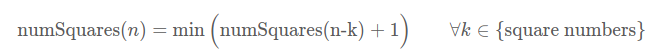
\includegraphics[width=300pt]{perfect-squares-dp.png}\\
\figcaption{Perfect Squares}\label{fig:perfect-squares-dp}
\end{center}

\begin{Code}
// LeetCode
// 時間複雜度O(n*sqtr(n)),空間複雜度O(n)
class Solution {
public:
    int numSquares(int n) {
        vector<int> dp(n+1, INT_MAX);
        // bottom case
        dp[0] = 0;

        // pre-calculate the square numbers.
        int max_square_index = (int) sqrt(n) + 1;
        vector<int> square_nums(max_square_index);

        for (int i = 1; i < max_square_index; ++i) {
            square_nums[i] = i * i;
        }

        for (int i = 1; i <= n; ++i) {
            for (int s = 1; s < max_square_index; ++s) {
                if (i < square_nums[s])
                    break;
                dp[i] = min(dp[i], dp[i - square_nums[s]] + 1);
            }
        }

        return dp[n];
    }
};
\end{Code}

\section{小結} %%%%%%%%%%%%%%%%%%%%%%%%%%%%%%
\label{sec:bfs-template}


\subsection{適用場景}

\textbf{輸入數據}:沒什麼特徵,不像深搜,需要有“遞歸”的性質。如果是樹或者圖,概率更大。

\textbf{狀態轉換圖}:樹或者DAG圖。

\textbf{求解目標}:求最短。


\subsection{思考的步驟}
\begin{enumerate}
\item 是求路徑長度,還是路徑本身(或動作序列)?
    \begin{enumerate}
    \item 如果是求路徑長度,則狀態裏面要存路徑長度(或雙隊列+一個全局變量)
    \item 如果是求路徑本身或動作序列
        \begin{enumerate}
            \item 要用一棵樹存儲寬搜過程中的路徑
            \item 是否可以預估狀態個數的上限?能夠預估狀態總數,則開一個大數組,用樹的雙親表示法;如果不能預估狀態總數,則要使用一棵通用的樹。這一步也是第4步的必要不充分條件。
        \end{enumerate}
    \end{enumerate}

\item 如何表示狀態?即一個狀態需要存儲哪些些必要的數據,才能夠完整提供如何擴展到下一步狀態的所有信息。一般記錄當前位置或整體局面。

\item 如何擴展狀態?這一步跟第2步相關。狀態裏記錄的數據不同,擴展方法就不同。對於固定不變的數據結構(一般題目直接給出,作為輸入數據),如二叉樹,圖等,擴展方法很簡單,直接往下一層走,對於隱式圖,要先在第1步裏想清楚狀態所帶的數據,想清楚了這點,那如何擴展就很簡單了。

\item 如何判斷重複?如果狀態轉換圖是一顆樹,則永遠不會出現迴路,不需要判重;如果狀態轉換圖是一個圖(這時候是一個圖上的BFS),則需要判重。
    \begin{enumerate}
    \item 如果是求最短路徑長度或一條路徑,則只需要讓“點”(即狀態)不重複出現,即可保證不出現迴路
    \item 如果是求所有路徑,注意此時,狀態轉換圖是DAG,即允許兩個父節點指向同一個子節點。具體實現時,每個節點要\textbf{“延遲”}加入到已訪問集合\fn{visited},要等一層全部訪問完後,再加入到\fn{visited}集合。
    \item 具體實現
        \begin{enumerate}
        \item 狀態是否存在完美哈希方案?即將狀態一一映射到整數,互相之間不會衝突。
        \item 如果不存在,則需要使用通用的哈希表(自己實現或用標準庫,例如\fn{unordered_set})來判重;自己實現哈希表的話,如果能夠預估狀態個數的上限,則可以開兩個數組,head和next,表示哈希表,參考第 \S \ref{subsec:eightDigits}節方案2。
        \item 如果存在,則可以開一個大布爾數組,來判重,且此時可以精確計算出狀態總數,而不僅僅是預估上限。
        \end{enumerate}
    \end{enumerate}

\item 目標狀態是否已知?如果題目已經給出了目標狀態,可以帶來很大便利,這時候可以從起始狀態出發,正向廣搜;也可以從目標狀態出發,逆向廣搜;也可以同時出發,雙向廣搜。
\end{enumerate}


\subsection{代碼模板}
廣搜需要一個隊列,用於一層一層擴展,一個hashset,用於判重,一棵樹(只求長度時不需要),用於存儲整棵樹。

對於隊列,可以用\fn{queue},也可以把\fn{vector}當做隊列使用。當求長度時,有兩種做法:
\begin{enumerate}
\item 只用一個隊列,但在狀態結構體\fn{state_t}裏增加一個整數字段\fn{level},表示當前所在的層次,當碰到目標狀態,直接輸出\fn{level}即可。這個方案,可以很容易的變成A*算法,把\fn{queue}替換為\fn{priority_queue}即可。
\item 用兩個隊列,\fn{current, next},分別表示當前層次和下一層,另設一個全局整數\fn{level},表示層數(也即路徑長度),當碰到目標狀態,輸出\fn{level}即可。這個方案,狀態裏可以不存路徑長度,只需全局設置一個整數\fn{level},比較節省內存;
\end{enumerate}

對於hashset,如果有完美哈希方案,用布爾數組(\fn{bool visited[STATE_MAX]}或\fn{vector<bool> visited(STATE_MAX, false)})來表示;如果沒有,可以用STL裏的\fn{set}或\fn{unordered_set}。

對於樹,如果用STL,可以用\fn{unordered_map<state_t, state_t > father}表示一顆樹,代碼非常簡潔。如果能夠預估狀態總數的上限(設為STATE_MAX),可以用數組(\fn{state_t nodes[STATE_MAX]}),即樹的雙親表示法來表示樹,效率更高,當然,需要寫更多代碼。


\subsubsection{如何表示狀態}

\begin{Codex}[label=bfs_common.h]
/** 狀態 */
struct state_t {
    int data1;  /** 狀態的數據,可以有多個字段. */
    int data2;  /** 狀態的數據,可以有多個字段. */
    // dataN;   /** 其他字段 */
    int action; /** 由父狀態移動到本狀態的動作,求動作序列時需要. */
    int level;  /** 所在的層次(從0開始),也即路徑長度-1,求路徑長度時需要;
                    不過,採用雙隊列時不需要本字段,只需全局設一個整數 */
    bool operator==(const state_t &other) const {
        return true;  // 根據具體問題實現
    }
};

// 定義hash函數

// 方法1:模板特化,當hash函數只需要狀態本身,不需要其他數據時,用這個方法比較簡潔
namespace std {
template<> struct hash<state_t> {
    size_t operator()(const state_t & x) const {
        return 0; // 根據具體問題實現
    }
};
}

// 方法2:函數對象,如果hash函數需要運行時數據,則用這種方法
class Hasher {
public:
    Hasher(int _m) : m(_m) {};
    size_t operator()(const state_t &s) const {
        return 0; // 根據具體問題實現
    }
private:
    int m; // 存放外面傳入的數據
};

/**
 * @brief 反向生成路徑,求一條路徑.
 * @param[in] father 樹
 * @param[in] target 目標節點
 * @return 從起點到target的路徑
 */
vector<state_t> gen_path(const unordered_map<state_t, state_t> &father,
        const state_t &target) {
    vector<state_t> path;
    path.push_back(target);

    for (state_t cur = target; father.find(cur) != father.end(); 
            cur = father.at(cur))
        path.push_back(cur);

    reverse(path.begin(), path.end());

    return path;
}

/**
 * 反向生成路徑,求所有路徑.
 * @param[in] father 存放了所有路徑的樹
 * @param[in] start 起點
 * @param[in] state 終點
 * @return 從起點到終點的所有路徑
 */
void gen_path(unordered_map<state_t, vector<state_t> > &father,
        const string &start, const state_t& state, vector<state_t> &path,
        vector<vector<state_t> > &result) {
    path.push_back(state);
    if (state == start) {
        if (!result.empty()) {
            if (path.size() < result[0].size()) {
                result.clear();
                result.push_back(path);
            } else if(path.size() == result[0].size()) {
                result.push_back(path);
            } else {
                // not possible
                throw std::logic_error("not possible to get here");
            }
        } else {
            result.push_back(path);
        }
        reverse(result.back().begin(), result.back().end());
    } else {
        for (const auto& f : father[state]) {
            gen_path(father, start, f, path, result);
        }
    }
    path.pop_back();
}
\end{Codex}


\subsubsection{求最短路徑長度或一條路徑}

\textbf{單隊列的寫法}

\begin{Codex}[label=bfs_template.cpp]
#include "bfs_common.h"

/**
 * @brief 廣搜,只用一個隊列.
 * @param[in] start 起點
 * @param[in] data 輸入數據
 * @return 從起點到目標狀態的一條最短路徑
 */
vector<state_t> bfs(state_t &start, const vector<vector<int>> &grid) {
    queue<state_t> q; // 隊列
    unordered_set<state_t> visited; // 判重
    unordered_map<state_t, state_t> father; // 樹,求路徑本身時才需要

    // 判斷狀態是否合法
    auto state_is_valid = [&](const state_t &s) { /*...*/ };

    // 判斷當前狀態是否為所求目標
    auto state_is_target = [&](const state_t &s) { /*...*/ };

    // 擴展當前狀態
    auto state_extend = [&](const state_t &s) {
        unordered_set<state_t> result;
        for (/*...*/) {
            const state_t new_state = /*...*/;
            if (state_is_valid(new_state) && 
                    visited.find(new_state) != visited.end()) {
                result.insert(new_state);
            }
        }
        return result;
    };

    assert (start.level == 0);
    q.push(start);
    while (!q.empty()) {
        // 千萬不能用 const auto&,pop() 會刪除元素,
        // 引用就變成了懸空引用
        const state_t state = q.front();
        q.pop();
        visited.insert(state);

        // 訪問節點
        if (state_is_target(state)) {
            return return gen_path(father, target); // 求一條路徑
            // return state.level + 1; // 求路徑長度
        }

        // 擴展節點
        vector<state_t> new_states = state_extend(state);
        for (const auto& new_state : new_states) {
            q.push(new_state);
            father[new_state] = state;  // 求一條路徑
            // visited.insert(state); // 優化:可以提前加入 visited 集合,
            // 從而縮小狀態擴展。這時 q 的含義略有變化,裏面存放的是處理了一半
            // 的節點:已經加入了visited,但還沒有擴展。別忘記 while循環開始
            // 前,要加一行代碼, visited.insert(start)
        }
    }

    return vector<state_t>();
    //return 0;
}
\end{Codex}


\textbf{雙隊列的寫法}
\begin{Codex}[label=bfs_template1.cpp]
#include "bfs_common.h"

/**
 * @brief 廣搜,使用兩個隊列.
 * @param[in] start 起點
 * @param[in] data 輸入數據
 * @return 從起點到目標狀態的一條最短路徑
 */
vector<state_t> bfs(const state_t &start, const type& data) {
    queue<state_t> next, current; // 當前層,下一層
    unordered_set<state_t> visited; // 判重
    unordered_map<state_t, state_t> father; // 樹,求路徑本身時才需要

    int level = -1;  // 層次

    // 判斷狀態是否合法
    auto state_is_valid = [&](const state_t &s) { /*...*/ };

    // 判斷當前狀態是否為所求目標
    auto state_is_target = [&](const state_t &s) { /*...*/ };

    // 擴展當前狀態
    auto state_extend = [&](const state_t &s) {
        unordered_set<state_t> result;
        for (/*...*/) {
            const state_t new_state = /*...*/;
            if (state_is_valid(new_state) && 
                    visited.find(new_state) != visited.end()) {
                result.insert(new_state);
            }
        }
        return result;
    };

    current.push(start);
    while (!current.empty()) {
        ++level;
        while (!current.empty()) {
            // 千萬不能用 const auto&,pop() 會刪除元素,
            // 引用就變成了懸空引用
            const auto state = current.front();
            current.pop();
            visited.insert(state);

            if (state_is_target(state)) {
                return return gen_path(father, state); // 求一條路徑
                // return state.level + 1; // 求路徑長度
            }

            const auto& new_states = state_extend(state);
            for (const auto& new_state : new_states) {
                next.push(new_state);
                father[new_state] = state;
                // visited.insert(state); // 優化:可以提前加入 visited 集合,
                // 從而縮小狀態擴展。這時 current 的含義略有變化,裏面存放的是處
                // 理了一半的節點:已經加入了visited,但還沒有擴展。別忘記 while
                // 循環開始前,要加一行代碼, visited.insert(start)
            }
        }
        swap(next, current); //!!! 交換兩個隊列
    }

    return vector<state_t>();
    // return 0;
}
\end{Codex}


\subsubsection{求所有路徑}

\textbf{單隊列}

\begin{Codex}[label=bfs_template.cpp]
/**
 * @brief 廣搜,使用一個隊列.
 * @param[in] start 起點
 * @param[in] data 輸入數據
 * @return 從起點到目標狀態的所有最短路徑
 */
vector<vector<state_t> > bfs(const state_t &start, const type& data) {
    queue<state_t> q;
    unordered_set<state_t> visited; // 判重
    unordered_map<state_t, vector<state_t> > father; // DAG

    auto state_is_valid = [&](const state_t& s) { /*...*/ };
    auto state_is_target = [&](const state_t &s) { /*...*/ };
    auto state_extend = [&](const state_t &s) {
        unordered_set<state_t> result;
        for (/*...*/) {
            const state_t new_state = /*...*/;
            if (state_is_valid(new_state)) {
                auto visited_iter = visited.find(new_state);

                if (visited_iter != visited.end()) {
                    if (visited_iter->level < new_state.level) {
                        // do nothing
                    } else if (visited_iter->level == new_state.level) {
                        result.insert(new_state);
                    } else { // not possible
                        throw std::logic_error("not possible to get here");
                    }
                } else {
                    result.insert(new_state);
                }
            }
        }

        return result;
    };

    vector<vector<string>> result;
    state_t start_state(start, 0);
    q.push(start_state);
    visited.insert(start_state);
    while (!q.empty()) {
        // 千萬不能用 const auto&,pop() 會刪除元素,
        // 引用就變成了懸空引用
        const auto state = q.front();
        q.pop();

        // 如果當前路徑長度已經超過當前最短路徑長度,
        // 可以中止對該路徑的處理,因為我們要找的是最短路徑
        if (!result.empty() && state.level + 1 > result[0].size()) break;

        if (state_is_target(state)) {
            vector<string> path;
            gen_path(father, start_state, state, path, result);
            continue;
        }
        // 必須挪到下面,比如同一層A和B兩個節點均指向了目標節點,
        // 那麼目標節點就會在q中出現兩次,輸出路徑就會翻倍
        // visited.insert(state);

        // 擴展節點
        const auto& new_states = state_extend(state);
        for (const auto& new_state : new_states) {
            if (visited.find(new_state) == visited.end()) {
                q.push(new_state);
            }
            visited.insert(new_state);
            father[new_state].push_back(state);
        }
    }

    return result;
}
\end{Codex}


\textbf{雙隊列的寫法}

\begin{Codex}[label=bfs_template.cpp]
#include "bfs_common.h"

/**
 * @brief 廣搜,使用兩個隊列.
 * @param[in] start 起點
 * @param[in] data 輸入數據
 * @return 從起點到目標狀態的所有最短路徑
 */
vector<vector<state_t> > bfs(const state_t &start, const type& data) {
    // 當前層,下一層,用unordered_set是為了去重,例如兩個父節點指向
    // 同一個子節點,如果用vector, 子節點就會在next裏出現兩次,其實此
    // 時 father 已經記錄了兩個父節點,next裏重複出現兩次是沒必要的
    unordered_set<string> current, next;
    unordered_set<state_t> visited; // 判重
    unordered_map<state_t, vector<state_t> > father; // DAG

    int level = -1;  // 層次

    // 判斷狀態是否合法
    auto state_is_valid = [&](const state_t &s) { /*...*/ };

    // 判斷當前狀態是否為所求目標
    auto state_is_target = [&](const state_t &s) { /*...*/ };

    // 擴展當前狀態
    auto state_extend = [&](const state_t &s) {
        unordered_set<state_t> result;
        for (/*...*/) {
            const state_t new_state = /*...*/;
            if (state_is_valid(new_state) && 
                    visited.find(new_state) != visited.end()) {
                result.insert(new_state);
            }
        }
        return result;
    };

    vector<vector<state_t> > result;
    current.insert(start);
    while (!current.empty()) {
        ++ level;
        // 如果當前路徑長度已經超過當前最短路徑長度,可以中止對該路徑的
        // 處理,因為我們要找的是最短路徑
        if (!result.empty() && level+1 > result[0].size()) break;

        // 1. 延遲加入visited, 這樣才能允許兩個父節點指向同一個子節點
        // 2. 一股腦current 全部加入visited, 是防止本層前一個節點擴展
        // 節點時,指向了本層後面尚未處理的節點,這條路徑必然不是最短的
        for (const auto& state : current)
            visited.insert(state);
        for (const auto& state : current) {
            if (state_is_target(state)) {
                vector<string> path;
                gen_path(father, path, start, state, result);
                continue;
            }

            const auto new_states = state_extend(state);
            for (const auto& new_state : new_states) {
                next.insert(new_state);
                father[new_state].push_back(state);
            }
        }

        current.clear();
        swap(current, next);
    }

    return result;
}
\end{Codex}

